\usetikzlibrary{arrows.meta,shapes.multipart}

\begin{frame}{what about 64-bit?}
\begin{itemize}
\item adds 8 more registers --- more bits for reg \#?
\item didn't change encoding for existing instructions, so\ldots
\item \myemph{instruction prefix} ``REX''
    \begin{itemize}
    \item 32-bit x86 already had many prefixes
    \end{itemize}
\item also selects 64-bit version of instruction
\end{itemize}
\end{frame}

\begin{frame}{REX prefix}
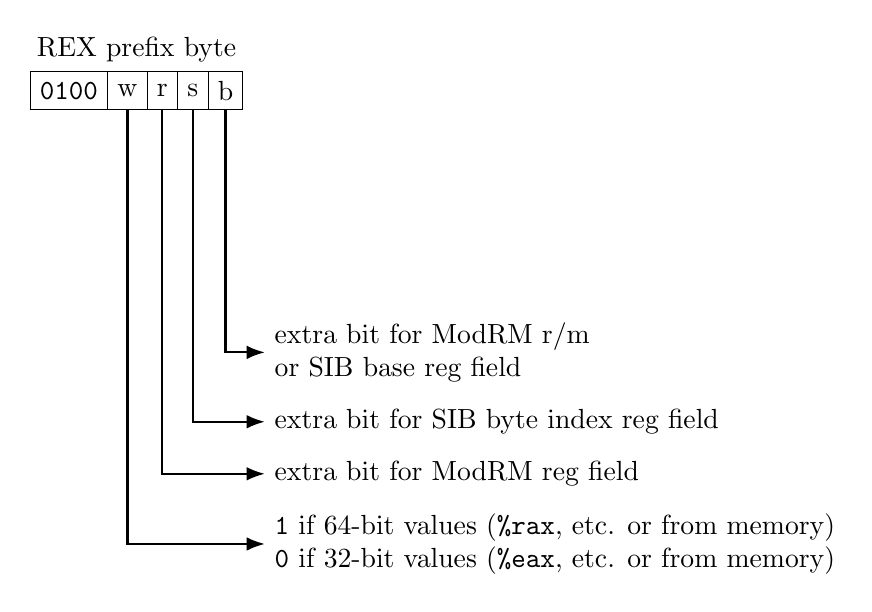
\begin{tikzpicture}
    \node[draw,rectangle split,rectangle split horizontal, rectangle split parts=5,
        label={north:REX prefix byte}] (rexbyte) {
        {\tt 0100}
        \nodepart{two}
        w
        \nodepart{three}
        r
        \nodepart{four}
        s
        \nodepart{five}
        b
    };
    \node[anchor=north west,align=left] (wExplain) at ([yshift=-5cm,xshift=.5cm]rexbyte.five south) {
        {\tt 1} if 64-bit values ({\tt \%rax}, etc. or from memory)\\
        {\tt 0} if 32-bit values ({\tt \%eax}, etc. or from memory)
    };
    \draw[thick,-Latex] (rexbyte.two south) |- (wExplain.west);
    \node[anchor=south west] (rExplain) at ([yshift=1mm]wExplain.north west) {
        extra bit for ModRM reg field
    };
    \draw[thick,-Latex] (rexbyte.three south) |- (rExplain.west);
    \node[anchor=south west] (sExplain) at ([yshift=1mm]rExplain.north west) {
        extra bit for SIB byte index reg field
    };
    \draw[thick,-Latex] (rexbyte.four south) |- (sExplain.west);
    \node[anchor=south west, align=left] (bExplain) at ([yshift=1mm]sExplain.north west) {
        extra bit for ModRM r/m \\ or SIB base reg field
    };
    \draw[thick,-Latex] (rexbyte.five south) |- (bExplain.west);
\end{tikzpicture}
%\vspace{.5cm}
%\item 4-bit constant 0100
%\item 1-bit ``w'': 1 if 64-bit operands
%\item 1-bit ``r'': extra bit for ModRM register number
%\item 1-bit ``s'': extra bit for SIB index register number
%\item 1-bit ``b'': extra bit for ``r/m'' or SIB index register number 
%    \begin{itemize}
%    \item or modify in-opcode register number
%    \end{itemize}
%\end{itemize}
\end{frame}

